\documentclass[runningheads]{../../../llncs}
\usepackage[paperheight=295mm,paperwidth=210mm]{geometry}
\usepackage{graphicx}
\usepackage{import}
\usepackage{kotex}
\usepackage[dvipsnames]{xcolor}
\usepackage{fancyvrb}
\usepackage{listings}
\usepackage{indentfirst}
\usepackage{tabularx}
\usepackage{underscore}
\usepackage{multicol}
\usepackage{enumitem}
\usepackage{menukeys}
\usepackage{amsmath}
\usepackage{clrscode3e} % https://www.ctan.org/pkg/clrscode3e?lang=en
\usepackage[numbers,square,super]{natbib}
\usepackage{inconsolata} % Inconsolata
\usepackage{mathptmx} % Times New Roman
\usepackage{minted}
\graphicspath{ {./images/} }
\lstset{basicstyle=\footnotesize\ttfamily,breaklines=true}
\renewcommand{\bibname}{참고문헌}
\setlength{\parindent}{1em}
\setlength{\parskip}{1em}
\linespread{1.2}
{\renewcommand{\arraystretch}{1.5}%
\setlength{\tabcolsep}{0.5em}%
\newenvironment{Figure}
  {\par\medskip\noindent\minipage{\linewidth}}
  {\endminipage\par\medskip}
\newcommand{\translation}[1]{\textsuperscript{#1}}
\newlist{algorithm}{enumerate}{10}
\setlist[algorithm]{label*=\arabic*.}
\setlist[algorithm,1]{label=\textbf{\arabic*}}
\setlist[algorithm,2]{label=\textbf{\alph*}}
\setlist[algorithm,3]{label=\textbf{\roman*}}
\setlist[algorithm,4]{label=(\arabic*)}
\setlist[algorithm,5]{label=(\alph*)}
\setlist[algorithm,6]{label=(\roman*)}
\makeatletter
\renewcommand\NAT@citesuper[3]{\ifNAT@swa
\if*#2*\else#2\NAT@spacechar\fi
\unskip\kern\p@\textsuperscript{\NAT@@open#1\if*#3*\else,\NAT@spacechar#3\fi\NAT@@close}%
   \else #1\fi\endgroup}
\makeatother
    
\usepackage{subfig}

\begin{document}

\title{CSE3013 (컴퓨터공학 설계 및 실험 I) \space \newline PRJ-2 테트리스 프로젝트 2주차 예비 보고서}
\author{서강대학교 컴퓨터공학과 박수현 (20181634)}
\institute{서강대학교 컴퓨터공학과}
\maketitle

\section{목적}
테트리스 게임에 랭킹을 추가한다.

\section{문제}
다음과 같은 쿼리를 효율적으로 처리할 수 있는 자료구조를 생각한다.
\begin{itemize}
    \item $(key, value)$의 2-tuple 원소 삽입
    \item 원소 삭제
    \item 정렬된 상태의 원소들에서 특정 인덱스 범위의 원소 조회
    \item 특정 $key$를 갖는 모든 $value$를 정렬된 상태로 조회
\end{itemize}

\subsection{링크드 리스트 (Linked List)}
교재에 소개된 대로 링크드 리스트를 이용해 랭킹을 관리할 수 있다. 링크드 리스트는 항상 정렬되어 있는 상태이다.

\subsubsection{삽입} 이 상황에서는 링크드 리스트가 정렬된 상태여야 하므로 원소를 특정한 위치에 삽입해야 한다.
링크드 리스트에서 원소를 특정 정렬된 위치에 삽입하는 것은 최악의 경우 마지막 원소까지 순회해야 하므로 $\mathcal{O}\left(n\right)$이다.

\begin{codebox}
\Procname{$\proc{LinkedList-Insert}(x)$}
\li Allocate new node $\id{newNode}$
\li $\attrib{newNode}{value} \gets x$
\li $\id{curr} \gets \id{head}$
\li \If $x > \attrib{curr}{value}$ \Then
\li     $\attrib{newNode}{link} \gets \id{head}$
\li     $\id{head} \gets \id{newNode}$
\li \Else
\li     \While $\attrib{curr}{link} \neq \const{null}$ and $x \leq \attribb{curr}{next}{value}$ \Do
\li         $\id{curr} \gets \attrib{curr}{link}$
        \End
\li $\attrib{newNode}{link} \gets \attrib{curr}{link}$
\li $\attrib{curr}{link} \gets\attrib{newNode}{link}$
    \End
\end{codebox}

\subsubsection{삭제} 링크드 리스트에서 $x$번째 원소를 삭제하는 것은 $x$번째 원소까지 순회하므로 $\mathcal{O}\left(x\right)$이다.

\begin{codebox}
\Procname{$\proc{LinkedList-Remove}(x)$}
\li $\id{curr} \gets \id{head}$
\li \If $x \isequal 1$ \Then
\li     $\id{head} \gets \attrib{head}{link}$
\li     Remove $\id{curr}$
\li \Else
\li     \For $i \gets 1$ \To $x-1$ \Do
\li         \If $\id{curr} \isequal \const{null}$ \Then
\li             \Error Array index out of range
\li         \Else
\li             $\id{curr} \gets \attrib{curr}{link}$
            \End
        \End
\li     $\id{next} \gets \attrib{curr}{link}$
\li     $\attrib{curr}{link} \gets \attrib{next}{link}$
\li     Remove $\id{next}$
    \End
\end{codebox}

\subsubsection{특정 범위의 원소 쿼리} $l$번째 원소부터 $r$번째 원소를 쿼리하는 것은 $r$번째 원소까지 순회하므로 $\mathcal{O}\left(r\right)$이다.

\begin{codebox}
\Procname{$\proc{LinkedList-Query}(l,\,r)$}

\li $\id{curr} \gets \id{head}$
\li \If $(1 \leq l \leq r \leq |\id{list}|) \neq \const{true}$ \Then
\li     \Error Array index out of range
    \End
\li $i \gets 1$
\li $\id{curr} \gets \id{head}$
\li \Repeat
\li     \If $l \leq i \leq r$ \Then
\li         Add $curr$ to query result
        \End
\li     $i \gets i + 1$
\li     $\id{curr} \gets \attrib{curr}{link}$
\li \Until $\id{curr} \isequal \const{null}$ or $i > r$
\end{codebox}

\newpage

\subsection{이진 탐색 트리 (Binary Search Tree)}

\begin{figure}[h]
    \begin{center}
        \resizebox{0.6\linewidth}{!}{%
        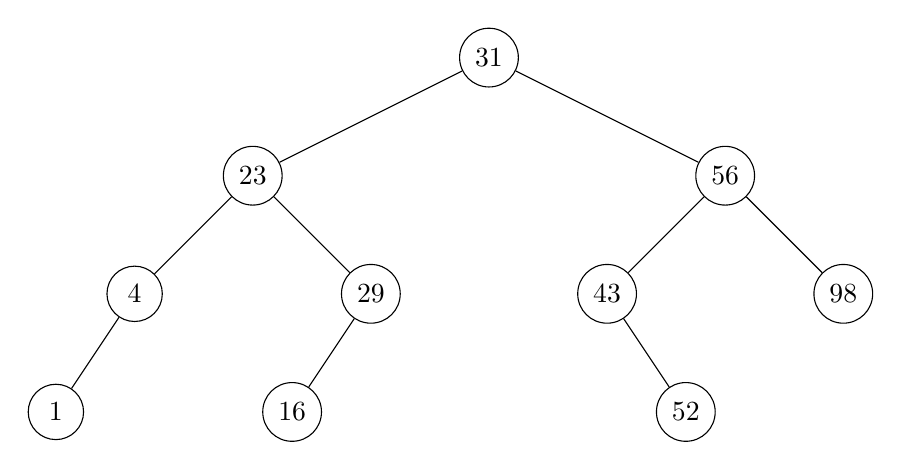
\begin{tikzpicture}[
            every node/.style = {minimum width = 2em, draw, circle},
            level/.style = {sibling distance = 60mm/#1}]
            \node {31}
            child {node {23} 
                child {node {4}
                    child {node {1}}
                    child {edge from parent[draw = none]}
                }
                child {node {29}
                    child {node {16}}
                    child {edge from parent[draw = none]}
                }
            }
            child {node {56}
                child {node {43}
                    child {edge from parent[draw = none]}
                    child {node {52}}
                }
                child {node {98}}
            };
        \end{tikzpicture}
        }
        \caption{이진 탐색 트리의 예시}
    \end{center}
\end{figure}

이진 탐색 트리는 이진 트리의 일종으로서, 각 노드의 왼쪽 서브트리는 해당 노드의 값보다 작은 노드들만, 오른쪽 서브트리는 해당 노드의 값보다 큰 노드들만을 포함하고 있는 트리를 말한다.

이진 탐색 트리에서 원소 삽입과 삭제에 걸리는 시간은 일반적으로 $\mathcal{O}\left(\log n\right)$이다.
또한 트리를 중위 순회($\mathcal{O}\left(n\right)$)할 경우 항상 정렬된 상태로 순회하게 되는 특징이 있다.
따라서 랭킹을 정렬된 상태로 조회해야 하는 쿼리들을 수행하는 데 효율적이다.

\begin{figure}[h]
    \centering
    \subfloat[최악의 경우의 이진 탐색 트리]{
        \resizebox{0.2\linewidth}{!}{%
        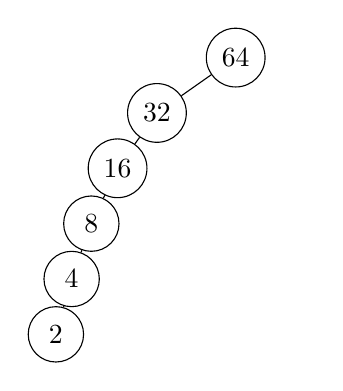
\begin{tikzpicture}[
            every node/.style = {minimum width = 2em, draw, circle},
            level/.style = {sibling distance = 20mm/#1}]
            \tikzset{level distance=20pt}
            \node {64}
            child {node {32} 
                child {node {16} 
                    child {node {8}
                        child {node {4}
                            child {node {2}}
                            child {edge from parent[draw = none]}
                        }
                        child {edge from parent[draw = none]}
                    }
                    child {edge from parent[draw = none]}
                }
                child {edge from parent[draw = none]}
            }
            child {edge from parent[draw = none]};
        \end{tikzpicture}
        }
        \label{fig:bst-worst}
    }%
    \qquad
    \subfloat[최적의 경우의 이진 탐색 트리]{
        \resizebox{0.2\linewidth}{!}{%
        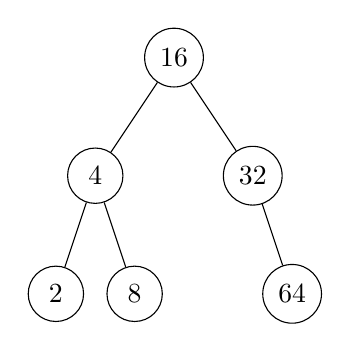
\begin{tikzpicture}[
            every node/.style = {minimum width = 2em, draw, circle},
            level/.style = {sibling distance = 20mm/#1}]
            \node {16}
            child {node {4} 
                child {node {2}}
                child {node {8}}
            }
            child {node {32} 
                child {edge from parent[draw = none]}
                child {node {64}}
            };
        \end{tikzpicture}
        }
    }%
    \caption{최악과 최적의 경우의 이진 탐색 트리}%
    \label{fig:bst}%
\end{figure}

하지만 Figure \ref{fig:bst-worst}의 경우처럼 이진 탐색 트리의 균형이 맞지 않을 경우 최대 $n$개의 노드를 순회해야 하므로
삽입/삭제 연산의 시간 복잡도는 링크드 리스트와 같아지게 된다. 여기에서 자가 균형 이진 탐색 트리\translation{self-balancing binary search tree}를 도입한다면
트리의 높이는 항상 $\left\lceil\log_2 n\right\rceil$가 되고, 최대 $\left\lceil\log_2 n\right\rceil$개의 노드만 순회하게 되므로 평균
$\mathcal{O}\left(\log n\right)$의 시간으로 원소를 삽입 및 삭제할 수 있게 된다.

자가 균형 이진 탐색 트리에는 AVL 트리, red-black 트리 등이 존재한다. C++ STL의 정렬 리스트 자료구조인 \mintinline{c++}{std::set}는 일반적으로
red-black 트리로 구현되어 있으므로 여기서도 red-black 트리(이하 RB 트리)를 이용한다.

\begin{figure}[h]
    \begin{center}
        \resizebox{0.65\linewidth}{!}{%
        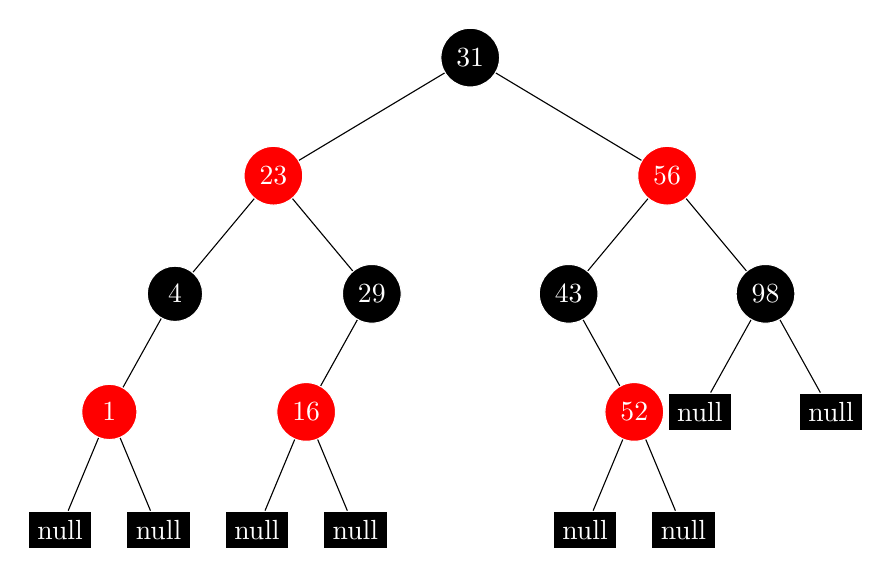
\begin{tikzpicture}[
            every node/.style = {minimum width = 2em, draw, circle, white},
            level/.style = {sibling distance = 50mm/#1}]
            \node[white,fill=black] {31}
            child {node[fill=red] {23} 
                child {node[fill=black] {4}
                    child {node[fill=red] {1}
                        child {node[fill=black,rectangle] {null}}
                        child {node[fill=black,rectangle] {null}}
                    }
                    child {edge from parent[draw = none]}
                }
                child {node[fill=black] {29}
                    child {node[fill=red] {16}
                        child {node[fill=black,rectangle] {null}}
                        child {node[fill=black,rectangle] {null}}
                    }
                    child {edge from parent[draw = none]}
                }
            }
            child {node[fill=red] {56}
                child {node[fill=black] {43}
                    child {edge from parent[draw = none]}
                    child {node[fill=red] {52}
                        child {node[fill=black,rectangle] {null}}
                        child {node[fill=black,rectangle] {null}}
                    }
                }
                child {node[fill=black] {98}
                    child {node[fill=black,rectangle] {null}}
                    child {node[fill=black,rectangle] {null}}
                }
            };
        \end{tikzpicture}
        }
        \caption{Red-black 트리의 예시}
    \end{center}
\end{figure}


RB 트리는 이진 탐색 트리에 더해 다음과 같은 성질들이 추가로 적용되는 트리이다.
\begin{itemize}
    \item 노드는 null일 수 있다.
    \item 각 노드의 색은 빨강, 검정 중 하나이다. 루트 노드나 null 노드는 항상 검정색이다.
    \item 어떤 노드가 빨강색일 경우 자식 노드는 모두 검정색이다.
    \item 임의의 노드에서 리프 노드까지의 모든 경로에는 같은 수의 검정 노드가 있다.
\end{itemize}
루트에서 리프 노드까지의 최단 경로가 모두 검정 노드로만 구성되어 있다고 했을 때, 최장 경로는 검정 노드와 빨강 노드가 번갈아 나오는 경로가 된다.
임의의 노드에서 리프 노드까지의 모든 경로에는 같은 수의 검정 노드가 있다고 했고, 빨강 노드의 자식은 무조건 검정 노드이므로
모든 경로에 대해 최장 경로의 거리는 최단 경로의 거리의 두 배 이상이 될 수 없게 된다.

각 노드마다 서브트리의 크기를 전처리해 추가로 저장해 주도록 한다.

삽입, 삭제 연산을 다루기 전에 우선 RB 트리의 성질들을 만족하게 하기 위해 연결 구조를 바꾸는 연산들을 정의한다. 모두 $\mathcal{O}\left(1\right)$ 연산들이다.

\proc{BST-Left-Rotate}: 노드 $x$의 위치로 $x$의 오른쪽 자식을 옮긴다.
\begin{codebox}
\Procname{$\proc{BST-Left-Rotate}(x)$}
\li \If $x$ has left child \Then
\li \Return
    \End
\li $y \gets \attrib{x}{right}$
\li $\attrib{x}{size} \gets \attrib{x}{left}{size} + \attrib{y}{left}{size} + 1$
\li $\attrib{y}{size} \gets \attrib{x}{size} + \attribb{y}{right}{size} + 1$
\li $\attrib{x}{right} \gets \attrib{y}{left}$
\li \If $\attrib{y}{left} \neq \const{null}$ \Then
\li     $\attribb{y}{left}{parent} \gets x$
    \End
\li $\attrib{y}{parent} \gets \attrib{y}{parent}$
\li \If $\attrib{x}{parent} \isequal \const{null}$ \Then
\li     $root \gets y$
\li \ElseIf $x \isequal \attribb{x}{parent}{left}$ \Then
\li     $\attribb{x}{parent}{left} \gets y$
\li \ElseNoIf
\li     $\attribb{x}{parent}{right} \gets y$
    \End
\li $\attrib{y}\id{left} \gets x$
\li $\attrib{x}\id{parent} \gets y$
\end{codebox}

\proc{BST-Right-Rotate}: 노드 $x$의 위치로 $x$의 왼쪽 자식을 옮긴다.
\begin{codebox}
\Procname{$\proc{BST-Right-Rotate}(x)$}
\li \If $x$ has right child \Then
\li \Return
    \End
\li $y \gets \attrib{x}{left}$
\li $\attrib{x}{size} \gets \attribb{x}{right}{size} + \attribb{y}{right}{size} + 1$
\li $\attrib{y}{size} \gets \attrib{x}{size} + \attribb{y}{left}{size} + 1$
\li $\attrib{x}{left} \gets \attrib{y}{right}$
\li \If $\attrib{y}{right} \neq \const{null}$ \Then
\li     $\attribb{y}{right}{parent} \gets x$
    \End
\li $\attrib{y}{parent} \gets \attrib{y}{parent}$
\li \If $\attrib{x}{parent} \isequal \const{null}$ \Then
\li     $root \gets y$
\li \ElseIf $x \isequal \attribb{x}{parent}{right}$ \Then
\li     $\attribb{x}{parent}{right} \gets y$
\li \ElseNoIf
\li     $\attribb{x}{parent}{left} \gets y$
    \End
\li $\attrib{y}\id{right} \gets x$
\li $\attrib{x}\id{parent} \gets y$
\end{codebox}

\proc{BST-Transplant}: $u$의 서브트리를 $v$의 서브트리로 대체한다.

\begin{codebox}
\Procname{$\proc{BST-Transplant}(u,\,v)$}
\li \If $\attrib{u}{parent} \isequal \const{null}$ \Then
\li     $\id{root} \gets v$
\li \ElseIf $u \isequal \attribb{u}{parent}{left}$ \Then
\li     $\attribb{u}{parent}{left} \gets v$
\li \ElseNoIf
\li     $\attribb{u}{parent}{right} \gets v$
    \End
\li $\attrib{v}{parent} \gets \attrib{u}{parent}$
\end{codebox}

$i$번째 순위의 노드를 가져오는 연산을 추가로 정의한다. DFS와 비슷한 식으로 탐색하며, 최대 $\left\lceil\log_2 n\right\rceil$개의 노드만 순회하므로
시간 복잡도는 $\mathcal{O}\left(\log n\right)$이다.

\proc{BST-Get}: $i$번째 순위의 노드를 가져온다.

\begin{codebox}
\Procname{$\proc{BST-Get}(u,\,i)$}
\li \If $i < \attribb{u}{left}{size}$ \Then
\li     \Return $\proc{BST-Get}(\attrib{u}{left},\,i)$
\li \ElseIf $i > \attribb{u}{left}{size}$ \Then
\li     \Return $\proc{BST-Get}(\attrib{u}{right},\,i-\attribb{u}{left}{size}-1)$
\li \ElseNoIf
\li     \Return $x$
    \End
\li $\attrib{v}{parent} \gets \attrib{u}{parent}$
\end{codebox}

\newpage

\subsubsection{삽입} 새 데이터를 갖는 빨강색 노드를 맨 밑에 삽입하고 트리의 성질에 맞도록 노드들을 재배치한다.
\proc{BST-Insert}에서 탐색 과정에 최악의 경우 트리의 높이만큼 탐색하고, 또 \proc{BST-Insert-Revalidate}에서 최악의 경우
루트로 두 칸씩 되돌아면서 $\dfrac{\mbox{트리의 높이}}{2}$만큼 탐색하므로 시간 복잡도는 $\mathcal{O}\left(\log n\right)$이다.

\begin{codebox}
\Procname{$\proc{BST-Insert}(u)$}
\li $y \gets \const{null}$
\li $x \gets root$
\li $\attrib{u}{size} \gets 1$
\li \While $x \neq \const{null}$ \Do
\li     $\attrib{x}{size} \gets \attrib{x}{size} + 1$
\li     $y \gets x$
\li     \If $\attrib{u}{key} < \attrib{x}{key}$ \Then
\li         $x \gets \attrib{x}{left}$
\li     \ElseNoIf
\li         $x \gets \attrib{x}{right}$
        \End
    \End
\li $\attrib{u}{parent} \gets y$
\li \If $y \isequal \const{null}$ \Then
\li     $\id{root} \gets u$
\li \ElseIf $\attrib{u}{key} < \attrib{y}{key}$ \Then
\li     $\attrib{y}{left} \gets u$
\li \ElseNoIf
\li     $\attrib{y}{right} \gets u$
    \End
\li $\attrib{u}{left} \gets \const{null}$, $\attrib{u}{right} \gets \const{null}$, $\attrib{u}{color} \gets \const{red}$ 
\li $\proc{BST-Insert-Revalidate}(u)$
\li $\id{size} \gets \id{size} + 1$
\end{codebox}

\newpage
    
\begin{codebox}
\Procname{$\proc{BST-Insert-Revalidate}(u)$}
\li \While $\attrib{u}{color} \isequal \const{red}$ \Do
\li     \If $\attrib{u}{parent} \isequal \attribbb{u}{parent}{parent}{right}$ \Then
\li         $v = \attribbb{u}{parent}{parent}right$
\li         \If $\attrib{v}{color} \isequal \const{red}$ \Then
\li             $\attribb{u}{parent}{color} \gets \const{black}$
\li             $\attrib{v}{color} \gets \const{black}$
\li             $\attribbb{u}{parent}{parent}{color} \gets \const{red}$
\li             $u \gets \attribb{u}{parent}{parent}$
\li         \ElseNoIf
\li             \If $u \isequal \attribb{u}{parent}{right}$ \Then
\li                 $u \gets \attrib{u}{parent}$
\li                 $\proc{BST-Left-Rotate}(u)$
                \End
\li             $\attribb{u}{parent}{color} \gets \const{black}$
\li             $\attribbb{u}{parent}{parent}{color} \gets \const{red}$
\li             $\proc{BST-Right-Rotate}(\attribb{u}{parent}{parent})$
            \End
\li     \ElseNoIf
\li         $v = \attribbb{u}{parent}{parent}left$
\li         \If $\attrib{v}{color} \isequal \const{red}$ \Then
\li             $\attribb{u}{parent}{color} \gets \const{black}$
\li             $\attrib{v}{color} \gets \const{black}$
\li             $\attribbb{u}{parent}{parent}{color} \gets \const{red}$
\li             $u \gets \attribb{u}{parent}{parent}$
\li         \ElseNoIf
\li             \If $u \isequal \attribb{u}{parent}{left}$ \Then
\li                 $u \gets \attrib{u}{parent}$
\li                 $\proc{BST-Right-Rotate}(u)$
                \End
\li             $\attribb{u}{parent}{color} \gets \const{black}$
\li             $\attribbb{u}{parent}{parent}{color} \gets \const{red}$
\li             $\proc{BST-Left-Rotate}(\attribb{u}{parent}{parent})$
            \End
        \End
    \End
\li $\attrib{root}{color} \gets \const{black}$
\end{codebox}

\newpage

\subsubsection{삭제} \proc{BST-Get}를 이용해 노드를 가져오고 일반적인 트리에서 원소를 삭제하듯이 삭제한다.
\proc{BST-Delete} 탐색 과정은 \proc{BST-Get}과 같은 시간이 걸리고, \proc{BST-Delete-Revalidate}에서 최악의 경우
마찬가지로 루트로 두 칸씩 되돌아면서 $\dfrac{\mbox{트리의 높이}}{2}$만큼 탐색하므로 시간 복잡도는 $\mathcal{O}\left(\log n\right)$이다.

\begin{codebox}
\Procname{$\proc{BST-Delete}(i)$}
\li $u \gets \proc{BST-Get}(\id{root}, i)$
\li $y \gets u$
\li $\id{originalColor} \gets \attrib{y}{color}$
\li \If $\attrib{u}{left} \isequal \const{null}$ \Then
\li     $x \gets \attrib{u}{right}$
\li     $\proc{BST-Transplant}(u,\,\attrib{u}{right})$
\li \ElseIf $\attrib{u}{right} \isequal \const{null}$ \Then
\li     $x \gets \attrib{u}{left}$
\li     $\proc{BST-Transplant}(u,\,\attrib{u}{left})$
\li \ElseNoIf
\li     $y \gets \mbox{(node with minimum index in }\attrib{u}{right}\mbox{)}$
\li     $x \gets \attrib{y}{right}$
\li     \If $\attrib{y}{parent} \isequal u$ \Then
\li         $\attrib{x}{parent} \gets y$
\li     \ElseNoIf
\li         $\proc{BST-Transplant}(y,\,\attrib{y}{right})$
\li         $\attrib{y}{right} \gets \attrib{u}{right}$
\li         $\attribb{y}{right}{parent} \gets y$
        \End
\li     $\proc{BST-Transplant}(u,\,y)$
\li     $\attrib{y}{left} \gets \attrib{u}{left}$, $\attrib{y}{parent} \gets y$, $\attrib{y}{color} \gets \attrib{u}{color}$
\li     \If $\id{originalColor} \isequal \const{black}$ \Then
\li         $\proc{BST-Delete-Revalidate}(x)$
        \End
    \End
\end{codebox}

\newpage

\begin{codebox}
\Procname{$\proc{BST-Delete-Revalidate}(x)$}
\li \While $x \neq \id{root}$ and $\attrib{x}{color} \isequal \const{black}$ \Do
\li     \If $x \isequal \attribb{x}{parent}{left}$ \Then
\li         $w \gets \attribb{x}{parent}{right}$
\li         \If $\attrib{w}{color} \isequal \const{red}$ \Then
\li             $\attrib{w}{color} \gets \const{black}$, $\attribb{w}{parent}{color} \gets \const{red}$
\li             $\proc{BST-Left-Rotate}(\attrib{x}{parent})$
\li             $w \gets \attribb{x}{parent}{right}$
            \End
\li         \If $\attribb{w}{left}{color} \isequal \const{black}$ and $\attribb{w}{right}{color} \isequal \const{black}$ \Then
\li             $\attrib{w}{color} \gets \const{red}$
\li             $x \gets \attrib{x}{parent}$
\li         \ElseNoIf
\li             \If $\attribb{w}{right}{color} \isequal \const{black}$ \Then
\li                 $\attribb{w}{left}{color} \gets \const{black}$, $\attrib{w}{color} \gets \const{red}$
\li                 $\proc{BST-Right-Rotate}(w)$
\li                 $w \gets \attribb{x}{parent}{right}$
                \End
\li             $\attrib{w}{color} \gets \attribb{w}{parent}{color}$
\li             $\attribb{x}{parent}{color} \gets \const{black}$, $\attribb{w}{right}{color} \gets \const{black}$
\li             $\proc{BST-Left-Rotate}(\attrib{x}{parent})$
\li             $x \gets \id{root}$
            \End
\li     \ElseNoIf
\li         $w \gets \attribb{x}{parent}{left}$
\li         \If $\attrib{w}{color} \isequal \const{red}$ \Then
\li             $\attrib{w}{color} \gets \const{black}$, $\attribb{w}{parent}{color} \gets \const{red}$
\li             $\proc{BST-Right-Rotate}(\attrib{x}{parent})$
\li             $w \gets \attribb{x}{parent}{left}$
            \End
\li         \If $\attribb{w}{right}{color} \isequal \const{black}$ and $\attribb{w}{left}{color} \isequal \const{black}$ \Then
\li             $\attrib{w}{color} \gets \const{red}$
\li             $x \gets \attrib{x}{parent}$
\li         \ElseNoIf
\li             \If $\attribb{w}{left}{color} \isequal \const{black}$ \Then
\li                 $\attribb{w}{right}{color} \gets \const{black}$, $\attrib{w}{color} \gets \const{red}$
\li                 $\proc{BST-Left-Rotate}(w)$
\li                 $w \gets \attribb{x}{parent}{left}$
                \End
\li             $\attrib{w}{color} \gets \attribb{w}{parent}{color}$
\li             $\attribb{x}{parent}{color} \gets \const{black}$, $\attribb{w}{left}{color} \gets \const{black}$
\li             $\proc{BST-Right-Rotate}(\attrib{x}{parent})$
\li             $x \gets \id{root}$
            \End
        \End
    \End
\li $\attrib{x}{color} \gets \const{black}$
\end{codebox}

\subsubsection{특정 범위의 원소 쿼리} $l$번째부터 $r$번째까지의 원소를 순회하도록 한다. 중위 순회한 결과값의 $l$부터 $r$번째 원소를
반환하면 된다. 시간 복잡도는 $\mathcal{O}\left(r\right)$아다. 다만 모든 $l$부터 $r$번째 인덱스마다 $\mathcal{O}\left(\log n\right)$의
\proc{BST-Get}을 호출하는 경우 시간 복잡도는 $\mathcal{O}\left(\left(r - l\right) \log n\right)$이므로
$r$보다 $\left(r - l + 1\right) \log n$이 현저히 작을 경우 이와 같은 방법으로 최적화할 수 있어 보인다.
아래 의사 코드는 최적화가 이뤄져 있지는 않다.

\begin{codebox}
\Procname{$\proc{BST-Query}(l,\,r)$}
\li \If $(1 \leq l \leq r \leq \id{size}) \neq \const{true}$ \Then
\li     \Error Array index out of range
    \End
\li Allocate new stack $s$
\li $\id{curr} \gets \id{root}$
\li \While $\id{curr} \neq \const{null}$ \Do
\li     Push $\id{curr}$ to $s$
\li     $\id{curr} \gets \attrib{curr}{left}$
    \End
\li \For $i = 1$ \To $r$ \Do
\li     \If $l \leq i$ \Then
\li         $\id{curr} \gets $ pop element from $s$
\li         Add $\id{curr}$ to query result
\li     \ElseNoIf
\li         Pop element from $s$
        \End
\li     $\id{curr} \gets \attrib{curr}{right}$
\li     \While $\id{curr} \neq \const{null}$ \Do
\li         Push $\id{curr}$ to $s$
\li         $\id{curr} \gets \attrib{curr}{left}$
        \End
    \End
\end{codebox}

\proc{BST-Get}의 공간 복잡도는 스택의 크기, 즉 $\mathcal{O}\left(r\right)$아다.

보고서에서 언급한 다른 모든 함수들의 공간 복잡도는 $\mathcal{O}\left(1\right)$이다.

\begin{thebibliography}{1}
    \bibitem{CLRS} T. H. Cormen, C. E. Leiserson, R. L. Rivest, C. Stein, \textit{Introduction
    to Algorithms}. Cambridge, MA: The MIT Press, 2009, pp. 287-338.
\end{thebibliography}

\end{document}
